\documentclass[a4paper,class=article,border=10pt,tikz]{standalone}

%mypackages
\usepackage{pythontex}
\usepackage{pgfplots}
\usepackage{amsmath}
\usepackage{titlesec}
\usepackage{tikz}
\usetikzlibrary{shapes.geometric}
\usetikzlibrary{positioning}
\usetikzlibrary{snakes,calc,positioning,patterns,angles,quotes,decorations.pathmorphing,decorations.markings}
% \titleformat{<command>}[<shape>]{<format>}{<label>}{<sep>}{<before-code>}[<after-code>]
%\titleformat{\section}{\normalfont\Large\bfseries}{\thesection.}{10pt}{}
% \titlespacing{<command>}{<left>}{<before-sep>}{<after-sep>}
%\titlespacing{\section}{0pt}{14pt}{7pt}

%\titleformat{\subsection}{\normalfont\itshape}{\thesubsection.}{10pt}{}
%\titlespacing{\subsection}{0pt}{12pt}{6pt}
% set font encoding for PDFLaTeX, XeLaTeX, or LuaTeX
\usepackage{ifxetex,ifluatex}
\if\ifxetex T\else\ifluatex T\else F\fi\fi T%
  \usepackage{fontspec}
\else
  \usepackage[T1]{fontenc}
  \usepackage[utf8]{inputenc}
  \usepackage{lmodern}
\fi

\usepackage{hyperref}


\title{Title of Document}
\author{Name of Author}

% Enable SageTeX to run SageMath code right inside this LaTeX file.
% http://doc.sagemath.org/html/en/tutorial/sagetex.html
% \usepackage{sagetex}

% Enable PythonTeX to run Python – https://ctan.org/pkg/pythontex
% \usepackage{pythontex}

\begin{document}

 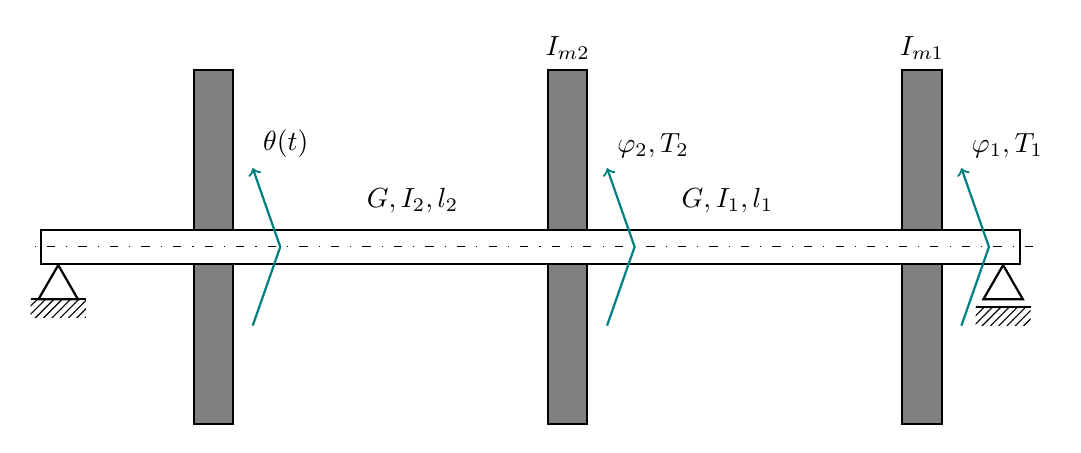
\begin{tikzpicture}

    \tikzstyle{ground}=[fill,pattern=north east lines,draw=none,minimum width=0.75cm,minimum height=0.3cm]
     \tikzstyle{close}=[draw=none,minimum width=0.75cm,minimum height=0.3cm]
      \coordinate (origo) at (0,0);

\node (I_1) [fill=gray,draw,outer sep=0pt,thick,minimum width=0.5cm,xshift=-0.03cm, minimum height=4.5cm,xshift=-1cm,label=above:{$I_{m1}$}]  at (origo) {};
\node (I_2) [fill=gray,draw,outer sep=0pt,thick,minimum width=0.5cm, minimum height=4.5cm,xshift=-4.5cm,label=above:{$I_{m2}$}]  at (I_1) {};
\node (I_0) [fill=gray,draw,outer sep=0pt,thick,minimum width=0.5cm, minimum height=4.5cm,xshift=-9cm]  at (I_1) {};




\draw[thick,double=white,double distance=0.4cm,line cap=rect] (origo) node (start){} --++(-3cm,0) node[xshift=-0.5cm,above=+0.3cm] (Label1){$G,I_1, l_1$} -- ++ (-1cm,0) node (P_load){} -- ++ (-2.5cm,0) node[xshift=-1cm,above=+0.3cm] (Label2){$G,I_2, l_2$} -- ++ (-5.5cm,0) node (shaft_end){};

\draw [thin, loosely dashdotted] ([xshift=0.25cm]start.east) --([xshift=-0.25cm]shaft_end.west);

% \node (wall_1) [ground,anchor=east,xshift=-12.21cm,yshift=0cm,minimum height=2cm ,minimum width=0.4cm] at (origo) {};

%\draw[thick] (wall_1.north east) -- (wall_1.south east);

\draw[thick, teal,->] (I_0)++(0.5cm,-1cm)  --++(0.35cm,1cm) --++ (-0.35cm,1cm) node[above right, black] {$\theta(t)$};

\draw[thick, teal,->] (I_1)++(0.5cm,-1cm)  --++(0.35cm,1cm) --++ (-0.35cm,1cm) node[above right, black] {${\varphi_{1}, T_1}$};

\draw[thick, teal,->] (I_2)++(0.5cm,-1cm)  --++(0.35cm,1cm) --++ (-0.35cm,1cm) node[above right, black] {${\varphi_{2}, T_2}$};


\draw [thick] ([yshift=-0.1cm]shaft_end.south) --++ (-60:0.5) --++(-0.5,0) node (support_end) {} --++ (60:0.5)  ;
\node (fixed_support) [ground,outer sep=0pt,thick,anchor=north west,xshift=-0.1cm,yshift=0cm,minimum height=0.1cm ,minimum width=0.7cm]  at (support_end) {};

\draw [thick] (fixed_support.north west) -- (fixed_support.north east);

\draw [thick] ([yshift=-0.1cm]start.south) --++ (-60:0.5) --++(-0.5,0)  node (support_start) {}  --++ (60:0.5);

\node (floating_support) [ground,outer sep=0pt,thick,anchor=north west,xshift=-0.1cm,yshift=-0.1cm,minimum height=0.05cm ,minimum width=0.7cm]  at (support_start) {};

\draw [thick] (floating_support.north west) -- (floating_support.north east);



\end{tikzpicture}

\end{document}
% \draw[<->,line width=1.5pt] (-0.5,0)--(0.5,0) node[midway,above]{$x_{e}(t)$};